    \section{Methodology}

    \subsection{Dependant Variables}\label{sec:dependent_variables}

    As mentioned in section \ref{sec:supervised_ml}, whenever any of the components of a feature vector's dimensionality, as defined in \ref{vector_dimensions}, changes, a new model has to be trained. The values for which various sets of HOG parameters will be tested in this investigation are listed in table \ref{table:dependent_variables}. Notice that the use of a "holistic" derivative mask, as introduced in section \ref{sec:deriv_mask} and implemented in appendix \ref{appendix:holistic_der_mask}, is also listed as a dependent variable. While the derivative mask which is used does not change a vector's dimensions it does change the vector's shape and, given the novel approach, it is nonetheless important to test how an SVM reacts to a differently shaped HOG descriptor. 

    \begin{table}
    \renewcommand{\arraystretch}{1.0}
    \begin{tabular}{@{} l @{\hspace{1cm}} l @{}}    
        \toprule
        \emph{Parameter} & \emph{Values}  \\\midrule
        Window Dimension Pairs ($W_h$,$W_w$)             & (100, 50), (128, 96), (128, 64), (112, 48)  \\ 
        Cell Histogram Bin Counts ($\omega$)              & 9, 13, 18  \\ 
        Cell Dimension Pairs ($c_w$,$c_h$)           & (4,4), (6,6), (8,8), (10,10)  \\ 
        Block Dimension Pairs ($b_w$,$b_h$)           & (1,1), (2,2), (3,3), (4,4)  \\ 
        Block Stride Dimension Pairs ($s_w$,$s_h$)              & (1,1), (2,2), (3,3)  \\ 
        Holistic Derivative Mask (appendix \ref{appendix:holistic_der_mask}) & True, False  \\\bottomrule
    \end{tabular}
    \caption{Dependent variables for the experiment}
    \label{table:dependent_variables}
    \end{table}

    The only restriction on the values in table \ref{table:dependent_variables} that can be combined to a set of HOG parameters is $b_w\ge s_w$ and $b_h\ge s_h$, since the use of blocks with stride values greater than block dimensions would result in certain cells being simply ignored for in the resultant feature vector $\vec{L}$. With the restriction, the number of different sets of values is given by $N$ in equation \ref{eq:number_sets}.

    \begin{equation}\label{eq:number_sets}
    \begin{split}
    N &= |\{(W_h, W_w)\}| \times |\{\omega\}| \times |\{(c_w, c_h)\}| \times 2 \times \sum_{\substack{b_w \geq s_w \\ b_h \geq s_h}} |\{(b_w, b_h)\}| \times |\{(s_w, s_h)\}|  \\
    &= 4 \times 3 \times 4 \times 2 \times 9  =864
    \end{split}
    \end{equation}

    \subsection{Data Sets}

    \subsubsection{Labeled Pedestrian Data Set Sources}

    Many past studies which have evaluated the HOG approach to feature detection have heavily \cite{piotrdollr_2012_crosstalk} or, in some cases \cite{zhou_2021_research}, solely relied on the INRIA pedestrian dataset \footnote{URL for the INRIA dataset (the original web page which provided the data set is, as of 2024 October 23rd, not accessible, thus a copy from \href{kaggle.com}{kaggle} is used): \url{https://www.kaggle.com/datasets/jcoral02/inriaperson}.}, as it has been the most popular data set for pedestrian detection algorithm evaluation \cite{dollar_2012_pedestrian} since HOG features were first introduced \cite{dalal_2005_histograms}. Nevertheless, there are flaws with the data set, mainly in the limited annotation: many people which appear in test images are not labelled, estimates of each person’s visibility are lacking, and there are no class labels for the regions of the images that contain ambiguous objects \cite{inria_improved}. Matteo Taiana et al introduced an improved iteration of INRIA with labelling that addresses the aforementioned issues and, as such, their improved INRIA data set \footnote{URL for the improved inria labels: \url{http://users.isr.ist.utl.pt/~mtaiana/data.html}.} will be used in this essay's experiment.

    Aside from the shortcomings of labelling in INRIA, the dataset is biased toward large, mostly unoccluded pedestrians \cite{dollar_2009_pedestrian}. The majority of people found in the dataset’s images are at a scale such that their limbs are 6 to 8 pixels wide \cite{dalal_2005_histograms}, which can undoubtedly introduce confirmation bias when attempting to evaluate the most performant cell size. As the goal of this investigation is to find a HOG descriptor that performs the best in real world environments, a greater variety of scales and occlusions will be introduced with the use of the more challenging and larger Caltech Pedestrian Dataset \cite{dollar_2009_pedestrian}, which contains richly annotated, low-resolution images of frequently occluded people. Images in real world applications may also include objects, like mannequins or statues, which closely resemble humanoid features, as previously shown in figure \ref{fig:manequin_features}. Neither INRIA nor the Caltech datasets contain such objects and thus a different dataset which addresses the range of false positive in pedestrian detection by providing labelled images with "person-like" objects \cite{karthika_2020_addressing} is also used in the investigation.

    \subsubsection{Caltech Data Set Transformation}\label{sec:caltech_trasnform}

    The PASCAL VOC challenges \cite{everingham_2009_pascal} introduced numerous standards in image classification, including the Pascal VOC labelling format, which has become the preferred scheme in many object classification applications, including pedestrian detection \cite{dollar_2012_pedestrian}. Both INRIA and the PnPLO (person-like) datasets abide this format, however the Caltech data set, since it's comprised of annotated videos rather than images, uses video bounding box labels \cite{mathworks_vbbLabeler}, which are especially useful for applications which involve tracking. This investigation, however, is only concerned with the detection of a pedestrian in an image, and because of that, the video (seq) files and video bounding box annotation (vbb) files are converted to images and Pascal VOC format xml files (appendix \ref{appendix:caltech_transform}). 

    Besides differences in annotation, the Caltech data set videos contain $\sim 250,000$ frames \cite{dollar_2009_pedestrian}, which vastly outnumbers the $1085$ images in INRIA \cite{dalal_2005_histograms} and $1339$ images in PnPLO \cite{karthika_2020_addressing}. Given both the great quantity of data in Caltech frames and the large amount of models (864 from equation \ref{eq:number_sets}) that would need to be trained on that data, it becomes apparent that to obtain a training time that is feasible for the computational resources that can be utilized in this investigation, the amount of frames needs to be reduced. 

    The total running time of the Caltech videos is $\sim 10\mathrm{h}$ \cite{dollar_2009_pedestrian}, this gives a frame per second rate of $\sim 7 \text{ frames}/\mathrm{s}$. Since a person is present in a video for $\sim 5 \mathrm{s}$ \cite{dollar_2009_pedestrian}, we can approximate that each identifiable individual will, on average, be present in $34 \text{ frames}$ and thus retaining only the $30$th frame of each video, as done in appendix \ref{appendix:caltech_30_frame}, should not incur a greatly significant cost on the amount of unique training data. By also removing frames that include the label "person?" (line 193 of appendix \ref{appendix:caltech_transform}), which denotes ambigious pedestrian figures, the sum of Caltech frames is significantly reduced to $8538$.

    \subsubsection{Window Size Samples}

    Dalal and Triggs proposed evaluating a detector by classifying cropped windows centered on pedestrians and comparing them to windows sampled at a fixed density from non-pedestrian images \cite{dalal_2005_histograms}, thereby eliminating the need to merge nearby detections, using methods like non maximal suppression (NMS), or other post-processing steps. Figure \ref{fig:dataset_high} shows a high level overview of per-window data set preparation.

    \begin{figure}
        \centering
        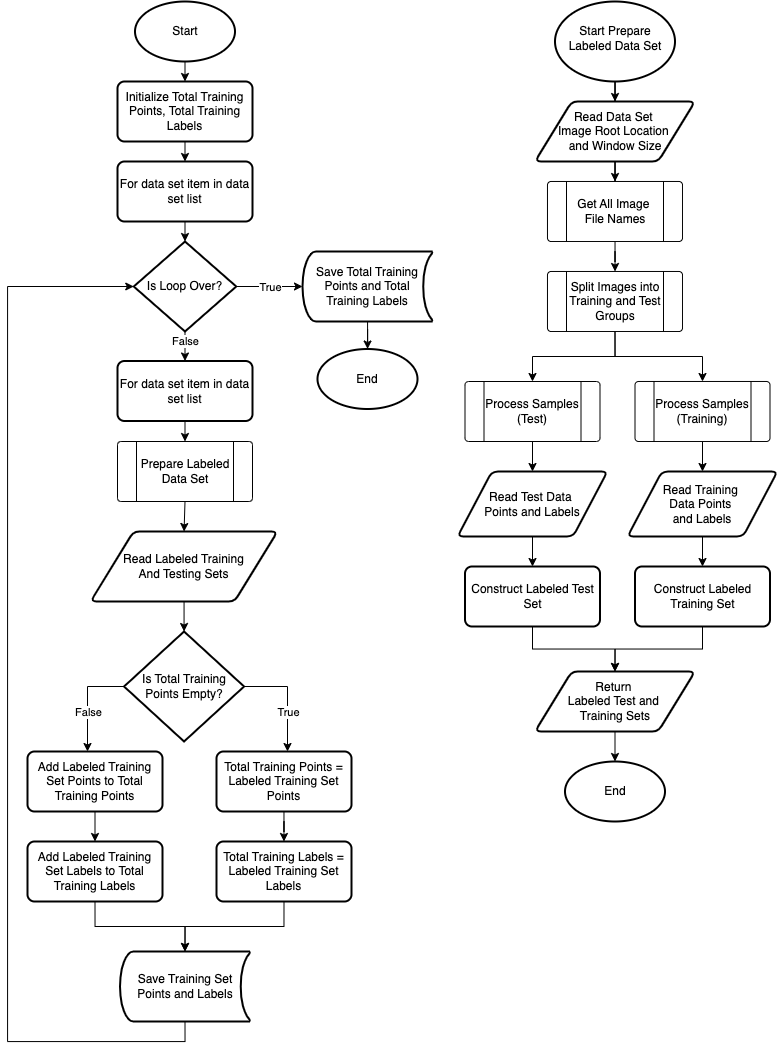
\includegraphics[width=0.75\linewidth]{images/ee_dataset_high.drawio.png}
        \caption{A high level overview flowchart of the process of initializing and saving the total training points and labels alongside each data set's testing points and labels}
        \label{fig:dataset_high}
    \end{figure}

    2 major concerns, however, have been raised with per-window evaluation: 
    \begin{enumerate}
        \item NMS may reduce the number of false positives at varying rates for different detection methods \cite{dollar_2009_pedestrian}
        \item The per-window scheme usually relies on the use of cropped positives (windows where a pedestrian is neatly bounded) and uncropped negatives (windows that are not specifically cropped to contain random objects or background scenery). Classifiers may exploit this window boundary effect as discriminative features leading to good per-window performance but poor performance in real life applications \cite{dollar_2009_pedestrian}
    \end{enumerate} 

    While concern nr. 1 should not impede this investigation's goal of finding the optimal HOG parameters, as each instance of HOG interacts in a similar fashion with NMS \cite{dalal_2005_histograms}, concern nr. 2 is addressed to some degree in line 162 of appendix \ref{appendix:dataset} by applying random value paddings to the bounding boxes that comprise positive samples. This process is further explained in figure \ref{fig:dataset_low}.

    \begin{figure}
        \centering
        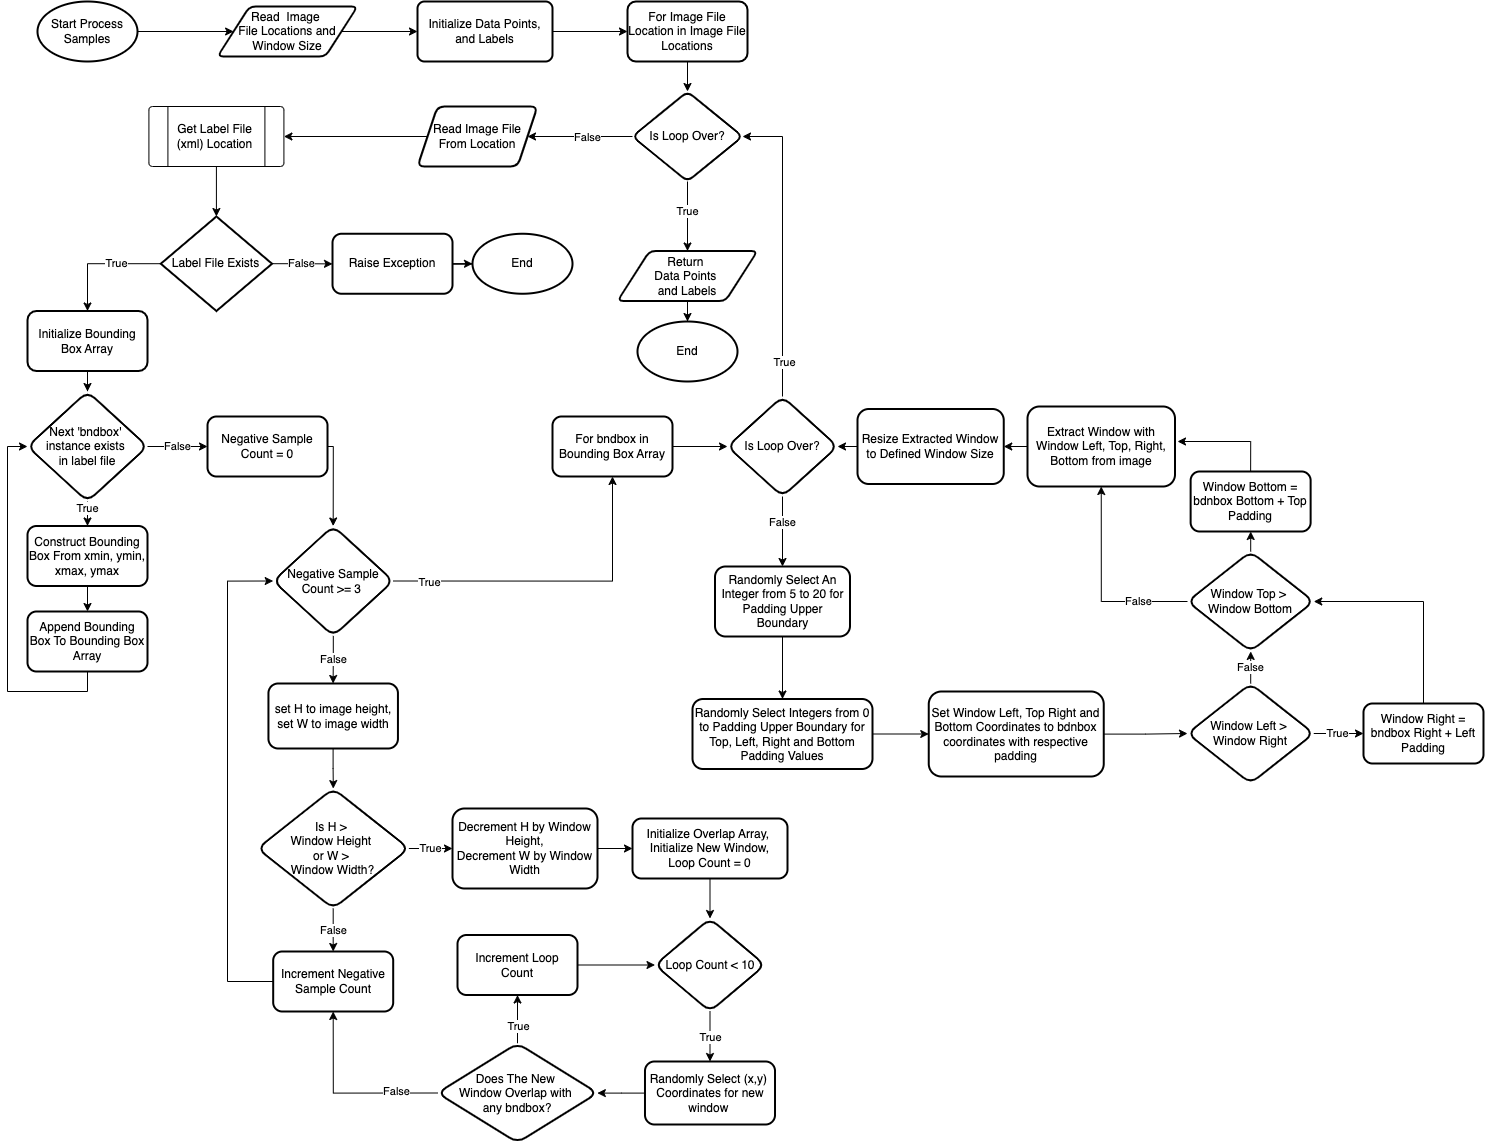
\includegraphics[width=\linewidth]{images/ee_dataset_low.drawio (1).png}
        \caption{A flowchart of the process of extracting the positive data samples (with some degree of random padding to avoid cropped positive bias) and the process of constructing negative samples }
        \label{fig:dataset_low}
    \end{figure}

    By using an 80/20\% training-testing data split, the number of images from section \ref{sec:caltech_trasnform} yields the numbers of different window size samples, as specified in table \ref{table:window_size_samples}

    \begin{table}[H]    
        \begin{minipage}{.5\linewidth}
        \renewcommand{\arraystretch}{1.0}
        \centering
            \begin{tabular}{@{} l @{\hspace{0.5cm}} l @{\hspace{0.5cm}} l @{}}    
                \toprule
                \emph{Window Set} & \emph{Positive} & \emph{Negative}  \\\midrule
                INRIA Testing & 361 & 543  \\ 
                Caltech Testing & 2195 & 2558  \\ 
                PnPLO Testing & 596 & 578  \\
                Total Training & 12794 & 14760 \\\bottomrule
            \end{tabular}
            \subcaption{Window Size (100, 50)}
        \end{minipage}%
        \begin{minipage}{.5\linewidth}
        \renewcommand{\arraystretch}{1.0}
        \centering
            \begin{tabular}{@{} l @{\hspace{0.5cm}} l @{\hspace{0.5cm}} l @{}}    
                \toprule
                \emph{Window Set} & \emph{Positive} & \emph{Negative}  \\\midrule
                INRIA Testing & 361 & 533  \\ 
                Caltech Testing & 2195 & 2548  \\ 
                PnPLO Testing & 596 & 475  \\
                Total Training & 12794 & 14185 \\\bottomrule
            \end{tabular}
            \subcaption{Window Size (128, 96)}
        \end{minipage}%

        \vspace{1cm} % Space between rows of minipages

        \begin{minipage}{.5\linewidth}
        \renewcommand{\arraystretch}{1.0}
        \centering
            \begin{tabular}{@{} l @{\hspace{0.5cm}} l @{\hspace{0.5cm}} l @{}}    
                \toprule
                \emph{Window Set} & \emph{Positive} & \emph{Negative}  \\\midrule
                INRIA Testing & 361 & 540  \\ 
                Caltech Testing & 2195 & 2554  \\ 
                PnPLO Testing & 596 & 535  \\
                Total Training & 12794 & 14511 \\\bottomrule
            \end{tabular}
            \subcaption{Window Size (128, 64)}
        \end{minipage}%
        \begin{minipage}{.5\linewidth}
        \renewcommand{\arraystretch}{1.0}
        \centering
            \begin{tabular}{@{} l @{\hspace{0.5cm}} l @{\hspace{0.5cm}} l @{}}    
                \toprule
                \emph{Window Set} & \emph{Positive} & \emph{Negative}  \\\midrule
                INRIA Testing & 361 & 543  \\ 
                Caltech Testing & 2195 & 2558  \\ 
                PnPLO Testing & 596 & 574  \\
                Total Training & 12794 & 14731 \\\bottomrule
            \end{tabular}
            \subcaption{Window Size (112, 48)}
        \end{minipage}%
    \caption{Positive And Negative Window Samples For Each Data Set at Each Window Size.}
    \label{table:window_size_samples}
    \end{table}

    \subsection{Evaluation Metrics}

    \subsubsection{The Basic Confusion Matrix Rates}
    In essence, all evaluation metrics of binary classification rely on the values of the confusion matrix, a $2 \times 2$ contingency table where the positive elements correctly classified as positives are called true positives (TP), the negative elements wrongly classified as positive are called false positives (FP), the negative elements correctly classified as negatives are called true negatives (TN), and the positive elements wrongly classified as negatives are called false negatives (FN), as shown in figure \ref{fig:conf_matrix}. \cite{chicco_eval_2023}. 

    \begin{figure}
        \centering
        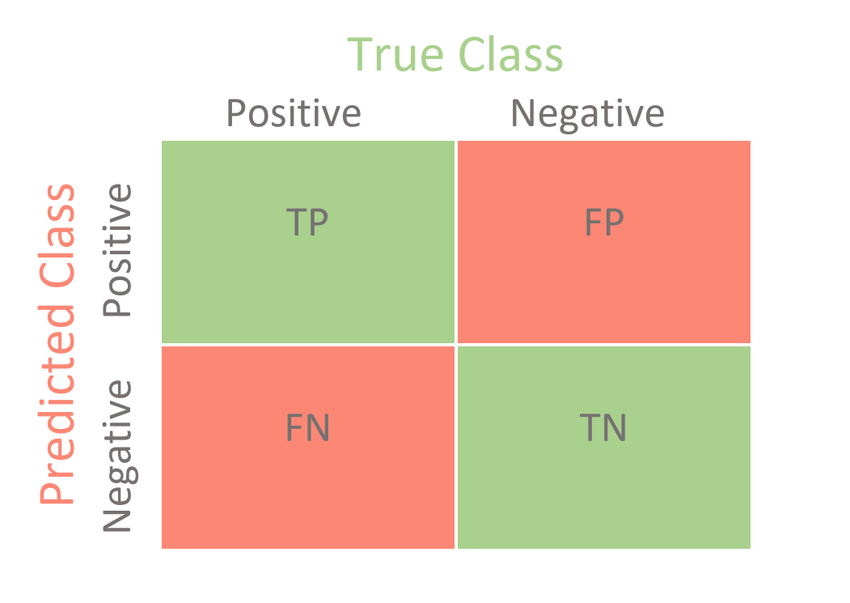
\includegraphics[width=0.5\linewidth]{images/conf_matrix.png}
        \caption{An example of a confusion matrix for binary classification. Source: \cite{conf_matrix}}
        \label{fig:conf_matrix}
    \end{figure}

    The four basic rates for confusion matrices are as follows \cite{chicco_eval_2023}:
    \begin{enumerate}
        \item Sensitivity, or True Positive Rate, $\mathrm{TPR}=\frac{\mathrm{TP}}{\mathrm{TP}+\mathrm{FN}}$

        \item Specificity, or True Negative Rate, $\mathrm{TNR}=\frac{\mathrm{TN}}{\mathrm{TN}+\mathrm{FP}}$
        
        \item Precision, or Positive Predictive Value, $\mathrm{PPV}=\frac{\mathrm{TP}}{\mathrm{TP}+\mathrm{FP}}$
        
        \item Negative Predictive Value, $\mathrm{PPV}=\frac{\mathrm{TN}}{\mathrm{TN}+\mathrm{FN}}$
    \end{enumerate} 

    \subsubsection{Confidence Threshold Curves}

    Many scoring classifiers produce a real-valued prediction score for each data point and, by assigning a particular threshold value $\tau$ a confusion matrix is generated for such a classifier \cite{chicco_jurman_2020_mcc_f1}. To summarize the confusion matrix, it is common to to plot one of the aforementioned four basic rates on a cartesian plane at varying $\tau$ values, like plotting a ROC curve (where TPR is plotted against the false positive rate $\mathrm{FPR}=\frac{\mathrm{TN}}{\mathrm{TN}+\mathrm{FP}}$) or the DET curve (FN rate against FP rate) which is more widespread in pedestrian detection literature \cite{dalal_2005_histograms} \cite{dollar_2012_pedestrian}. 

    However, unlike methods such as logistic regression \cite{cornell_log_regression_notes}, which classify a window into one of two classes by estimating the probability that the window belongs to each class, an SVM is not a "probabilistic" model as it simply plots the window's feature vector in a space separated by a hyperplane, and thus there's no probabilistic/scoring confidence $\tau$ involved. While it's possible to compute the probabilities of an SVMs prediction using cross-validation in Platt Scaling \cite{platt1999probabilistic}, the operation is known to be very expensive for large datasets \cite{scikit-learn_svm} alongside being inconsistent with the actual predictions of the SVM \cite{scikit-learn_svm}. Nevertheless, plots with varying $\tau$ values can be extremely informative \cite{martin1997det} \cite{scikit-learn_svm} and thus instead of "probabilities", the distances from each data point to the hyperplane are used as a sort of "confidence" value.

    \subsubsection{Matthew's Correlation Coefficient}

    While ROC curves (or their DET counterparts) alongside the scalar value of area under the ROC curve (AUC-ROC) are very widespread, they are also fundamentally flawed in that they ignore precision since, fundamentally, AUC-ROC only identifies how well a classifier separates the positive class from the negative class, not how accurate the separation is (a metric which is ever more important in a field like pedestrian detection). Historically, precision recall curves were used to account for the drawbacks of ROC \cite{chicco_jurman_2020_mcc_f1}. Quite recently, however, the Matthew's Correlation Coefficient has been proposed as a standard metric for validating biomedical image analysis by an international group of researchers in the field \cite{Maier_Hein_2024_mcc_proposal}, primarily because it is the only rate that maximizes all four of the aforementioned basic rates \cite{Maier_Hein_2024_mcc_proposal} \cite{chicco_eval_2023} \cite{chicco_jurman_2020_mcc_f1} and is claimed to be the most informative single score to establish the quality of a binary classifier prediction \cite{chicco_eval_2023}. Because of its discriminatory power, the MCC and a corresponding MCC-F1 curve (explained in more detail in figure \ref{fig:mcc_f1_example}) will be the primary evaluation metrics used in this investigation. 

    \begin{figure}
        \centering
        \includesvg[width=0.8\linewidth]{images/mcc_f1_example.svg}
        \caption{An example of an MCC-F1 curve. Unit-normalized Matthews correlation coefficient (MCC) plotted against the F1 score (the harmonic mean between precision and recall). The random line indicates that a random classifier can achieve a unit-normalized MCC of 0.5. The point of perfect performance is (1,1), representing an ideal classifier that correctly classifies every instance. Conversely, the point of worst performance is (0,0), attained by a classifier that misclassifies all instances. The best threshold point is the location on the curve that is nearest to (1,1). 5 various threshold $\tau$ values are scattered along the curve. Source: Image by Me, generated with code in appendix \ref{appendix:mcc_f1_curves}}
        \label{fig:mcc_f1_example}
    \end{figure}


    \begin{figure}
        $$\mathrm{MCC} = \frac{\mathrm{TP}\cdot\mathrm{TN}-\mathrm{FP}\cdot\mathrm{FN}}{\sqrt{(\mathrm{TP}+\mathrm{FP})\cdot(\mathrm{TP}+\mathrm{FN})\cdot(\mathrm{TN}+\mathrm{FP})\cdot(\mathrm{TN})+\mathrm{FN}}}$$ 
        \caption{The equation for Matthew's Correlation Coefficient. The values of MCC are bounded within the range $[-1;1]$, where 1 represents a perfect prediction, 0 represents random prediction and -1 total disagreement between prediction and observation. Refer to \cite{chicco_jurman_2020_mcc_f1} regarding the necessary normalization to make the MCC values bounded within $[0;1]$ so that they can be plotted against F1 scores (which themselves are bounded in $[0;1]$)}
    \end{figure}

    Nevertheless, since much of the literature on pedestrian detection and classification has historically relied on the aforementioned metrics of AUC-ROC, Average Precision and simple Accuracy \cite{dalal_2005_histograms} \cite{dollar_2012_pedestrian}, they are retained to facilitate direct and simple comparison with previous studies.

    \subsubsection{McNemar's Test for Pairwise Classifier Comparison}

    There are many ways to perform pairwise classifier comparison, such as conducting $5 \times 2$ Cross Validation (CV), which has historically been the preferred scheme in object classification \cite{dietterich_1998_mcnemar}. However, $5 \times 2$ CV, as the name implies, needs to be executed 10 times, while a test like McNemar's requires only a single execution. McNemar's test is also a more attractive choice as it performs increasingly better with larger datasets \cite{raschka_2018_mcnemar}. Additionally, it utilizes a version of the familiar confusion matrix, illustrated in Figure \ref{fig:confusion_mcnemar}.

    \begin{figure}
        \centering
        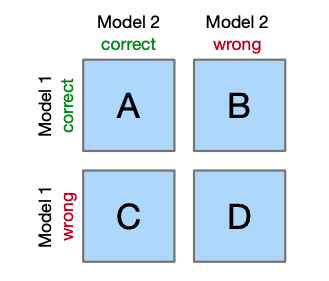
\includegraphics[width=0.5\linewidth]{images/mcnemar_matrix.png}
        \caption{Confusion matrix layout in the context of McNemar's test. Source: \cite{raschka_2018_mcnemar} Code for the construction of such a matrix can be found in appendix \ref{appendix:mcnemar}}
        \label{fig:confusion_mcnemar}
    \end{figure}

    McNemar's test checks if two classifiers have significantly different performance by comparing their disagreement on predictions in the confusion matrix. It calculates a p-value, the probability that the observed difference in performance is due to chance, based on a chi-square statistic \cite{dietterich_1998_mcnemar}. Typically, all p-values $\ge 0.05$ indicate that the difference between performance is not significant \cite{raschka_2018_mcnemar} \cite{dietterich_1998_mcnemar}. 

    % TODO: Should I talk more about p-value and the null hypothesis?

    \subsection{Model Preparation}

    As mentioned in sections \ref{§sec:supervised_ml} and \ref{sec:dependent_variables}, a data set has to be uniquely prepared for each of the different 864 SVM models. This is done in two steps: by first preprocessing each window sample and then computing the HOG features (data points) on which a model will be trained and tested.

    \subsubsection{Preprocessing: Grayscale Image Transformation}

    The only preprocessing step used in the original HOG paper was gamma/color normalization \cite{dalal_2005_histograms}. While the paper did show that there are modest variations in classifier accuracy depending on whether an RGB, LAB or grayscale color space is used, it was also shown that the difference in illuminance became even more negligible once block normalization was applied \cite{dalal_2005_histograms}. Thus, for the sake computational simplicity, 3-channeled data points are first transformed to grayscale color spaces.

    Given the rather ambiguous nature of assessing which specific method of RGB to grayscale conversion produces universally desirable outputs for all involved input images \cite{madk_2008_perceptual}, a simple and widely adopted color mapping defined in equation \ref{eq:colour_map} is used in appendix \ref{appendix:grayscale}

    \begin{equation}\label{eq:colour_map}
        Y \leftarrow 0.2125 \cdot R + 0.7154 \cdot G + 0.0721 \cdot B
    \end{equation}

    \subsubsection{Computing HOG Features}

    While an in depth explanation of how HOG features are computed was presented in section \ref{sec:hog}, there are a few notes to be made regarding the implementation of HOG in this investigation.

    Since neither the \href{https://scikit-image.org/}{scikit-image} nor \href{https://opencv.org/}{OpenCV} libraries provide an implementation of HOG which would allow changing the block stride values, a custom implementation of the algorithm can be found in appendix \ref{appendix:hog}, with figure \ref{fig:hog_flowchart} providing a technical overview. The two parts of the hog pipeline (from figure \ref{fig:hog_pipeline}) that have still been reused from \href{https://scikit-image.org/}{scikit-image} are the distribution of votes to histogram bins and block normalization, as shown in figure \ref{fig:hog_flowchart}. This is primarily because both parts are highly optimized using \href{https://cython.org/}{Cython}. Even while the votes are not distributed using equation \ref{eq:bin}, giving a time complexity of $\mathcal{O}(\omega \cdot c_h \cdot c_w)$ instead of $\mathcal{O}(c_h \cdot c_w)$, the speed of the library's Cython implementation outperforms anything that would be possible using regular python.

    \begin{figure}
        \centering
        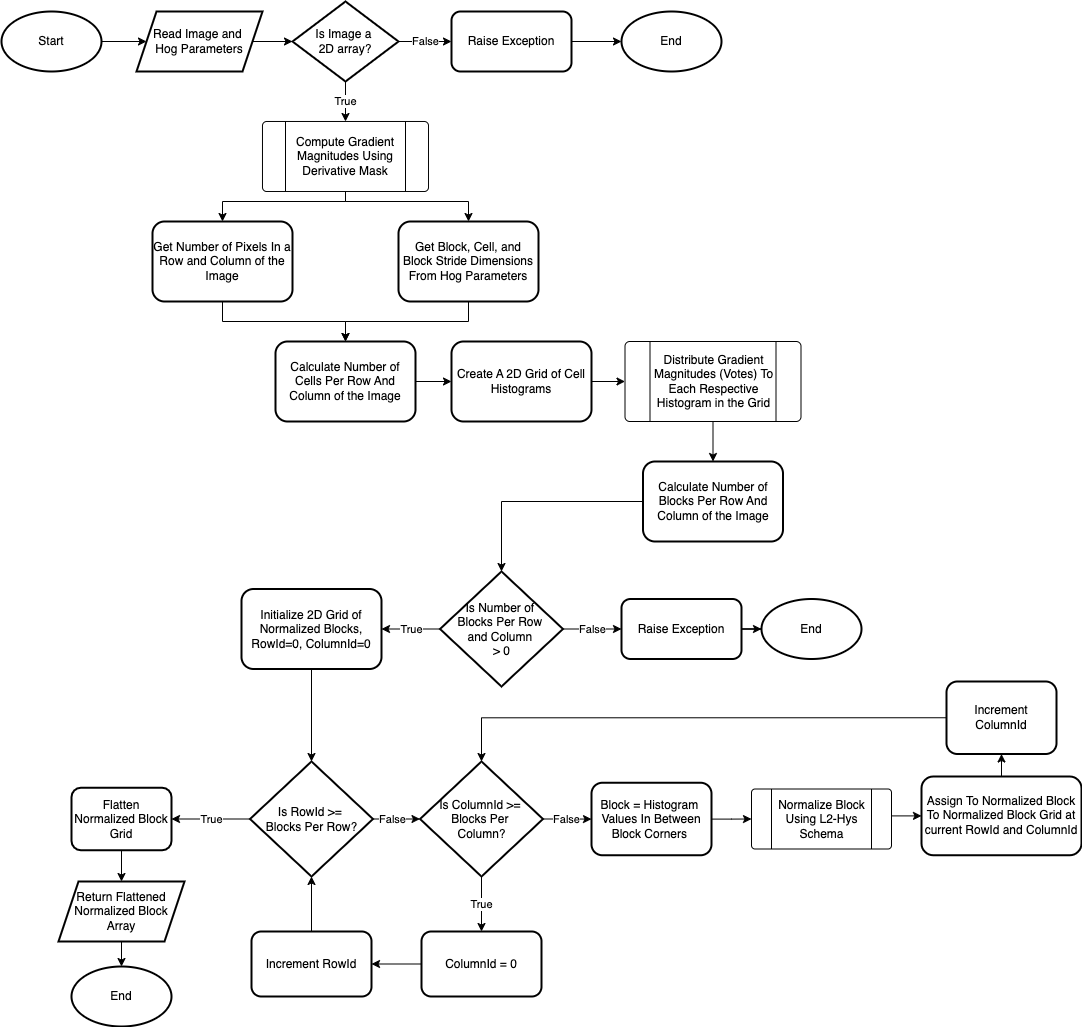
\includegraphics[width=0.85\linewidth]{images/ee_hog.drawio.png}
        \caption{A flowchart of the process of computing HOG features with custom block stride values}
        \label{fig:hog_flowchart}
    \end{figure}

    \subsubsection{Choosing an SVM}

    The primary factor driving the choice of SVM implementation is time of computation. Given the relatively large number of models that have to be trained on $\sim$ 27,000 samples, an implementation which is able to maximize the hyperplane's margin in the least amount of time while still maintaining relatively decent classification performance is a necessity. 

    The standard SVM implementation is LibSVM \cite{chang_lin_2011_libsvm} \cite{scikit-learn_svm}, however, it's training times scale quadratically with the number of samples \cite{scikit-learn_svm} (in practice it takes $\sim$ 1,600,000 \% more time to train an SVM with SMO as opposed to SGD \cite{sgd_leon}). The maintainers \href{https://scikit-learn.org/}{scikit-learn} recommend using either LibLinear or their own implementation of a linear SVM with stochastic gradient descent (SGD). SGD only uses a subset of samples when determining the cost function's, which, in this case, has inputs of §$||w||_{2}$ and $b$ from section \ref{sec:soft_constraint_svm}, gradient and the subsequent direction towards the global minima \cite{uc_berkeley_sgd}. This is in contrast to regular gradient descent (GD) which uses all samples for gradient calculation. As such, while training a model with SGD would be faster, we should also expect the SGD model to have worse performance guarantees than GD \cite{uc_berkeley_sgd}.

    In practice however, both LibLinear \footnote{LibLinear SVM docs: \url{https://scikit-learn.org/1.5/modules/generated/sklearn.svm.LinearSVC.html}} and an SVM with GDC \footnote{SVM with SGD docs: \url{https://scikit-learn.org/1.5/modules/generated/sklearn.linear_model.SGDClassifier.html}} exhibit essentially identical pedestrian classification performance, as evidenced by a McNemar's test p-value of $\sim$ 0.121, further comparisons are made in table \ref{tab:liblinear_vs_sgd_table} and figure \ref{fig:liblinear_vs_sgd_curve}.

    \begin{table}
        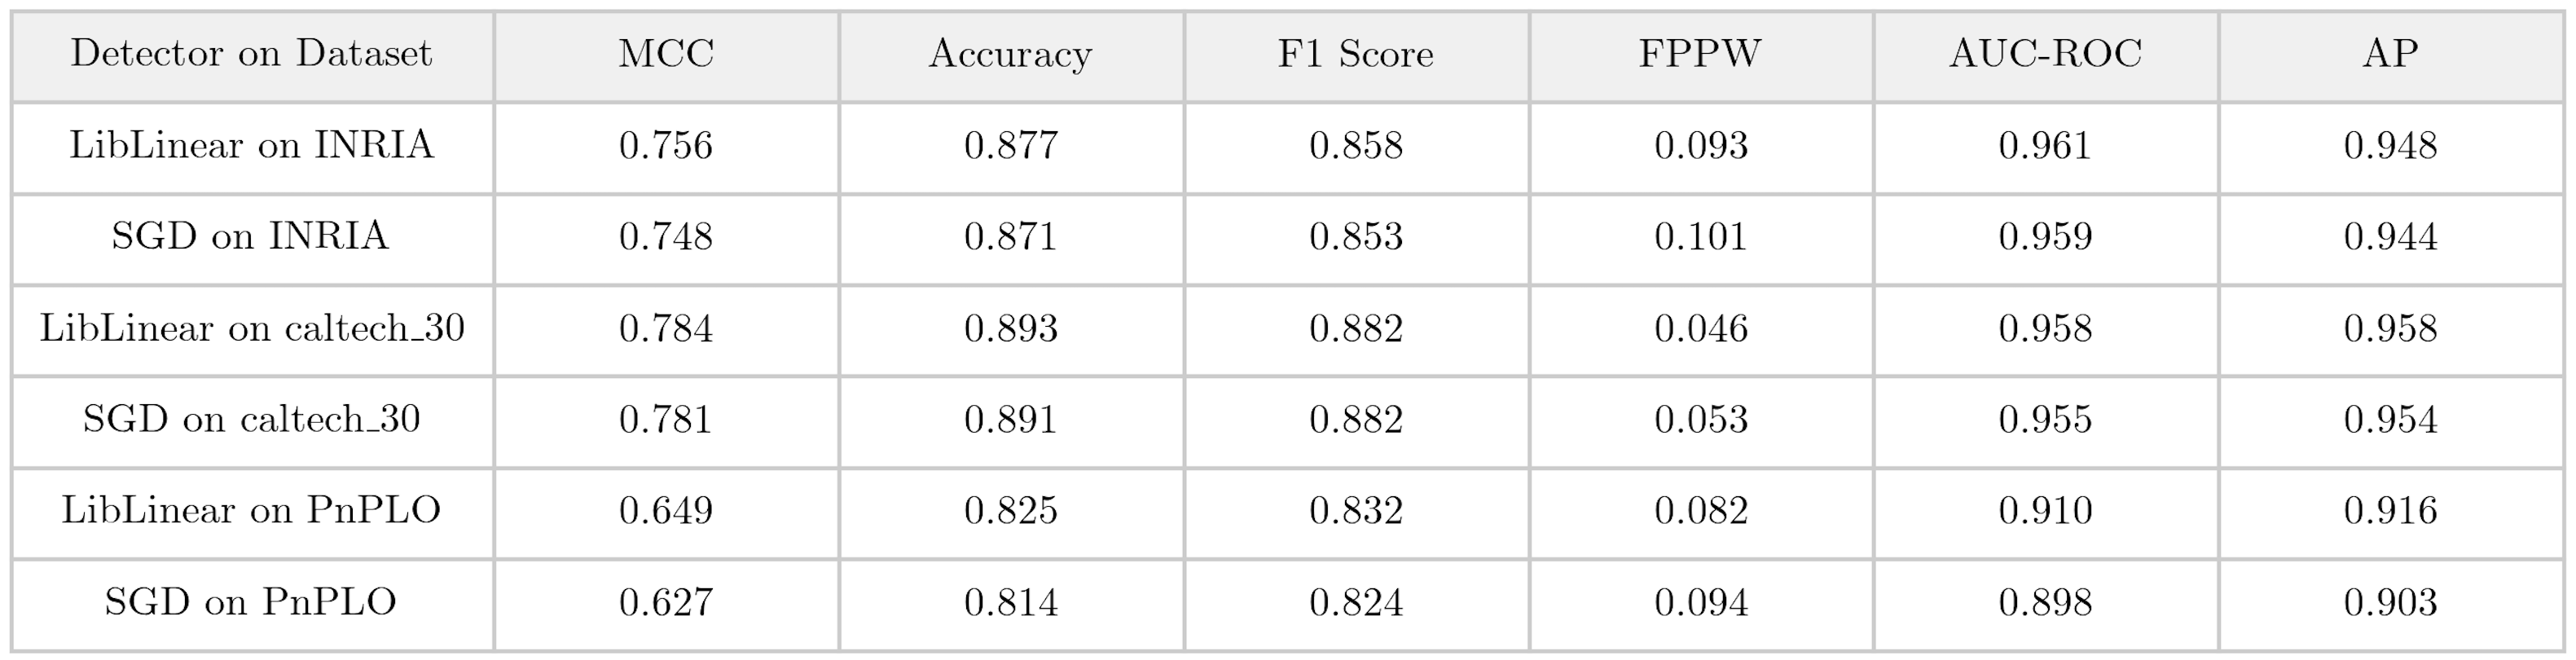
\includegraphics[width=\linewidth]{images/liblinear_vs_sgd_table.png}
        \caption{The evaluation metrics of a LinearSVC and SGDClassifier SVM implementations, trained on the standard HOG feature parameters \cite{dalal_2005_histograms}: $128\times64$ windows with $8\times8$ pixels per cell, $2\times2$ cells per block, $1\times1$ block strides. Source: Image by Me, generated with code in appendix \ref{appendix:evaluate_metrics}}
        \label{tab:liblinear_vs_sgd_table}. 
    \end{table}


    \begin{figure}
        \centering
        \includesvg[width=0.75\linewidth]{images/liblinear_vs_sgd_curve.svg}
        \caption{An MCC-F1 curve of both LinearSVC and SGDClassifier trained on the standard HOG feature parameters \cite{dalal_2005_histograms}. Notice that the best performing $\tau$ value for SGDClassifier is negative, as $\tau$ identifies the distance which allows a point to be classified as a positive. This relates to Soft Constraint SVMs mentioned in section \ref{sec:soft_constraint_svm}.}
        \label{fig:liblinear_vs_sgd_curve}
    \end{figure}

    \subsubsection{Training an SVM}

    The code in appendix \ref{appendix:training_svm} implements SVM training using SGDClassifier optimized through cross 5-fold validation (with GridSearchCV) \cite{cornell_hyperoptimization}, which systematically explores different regularization strength values (alpha). The search grid consists of 4 "soft" regularization parameters, as discussed in section \ref{sec:soft_constraint_svm}. This means that each SGDClassifier will be fitted a total of 20 times, with the best performing model (in terms of MCC) being saved for each set of HOG parameters. While the initial learning rate (eta$\theta$) is also a parameter that should be optimized, this investigation avoids the additional training overhead by using Leon Bottou's "optimal heuristic" for deriving the learning rate from alpha \cite{sgd_leon}.

    The majority of the training was performed on a linux-based system with an Intel Xeon CPU @ 2.20GHz (2 cores), 12.7GB of RAM, as provided by \href{https://colab.research.google.com/}{Google Colab}. Especially high dimensional HOG features (from figure \ref{fig:dimension_distribution}) tend to exceed the memory capacity of google colab's free tier, which is why the training for higher dimensional models was done on a local machine with an Intel Core i7 @ 2.6GHz (6 cores) and 32GB of RAM.

    \begin{figure}
        \includesvg[
            width=\linewidth,
        ]{dimension_distribution.svg}
        \caption{Kernel Density Estimation (KDE) of Dimension Values generated from various Histogram of Oriented Gradients (HOG) parameters. The blue line represents the KDE trend of the dimensions, while the red dots indicate the discrete dimension values calculated from different sets of HOG parameters. The most frequent number of dimensions is 3780, which is the number of dimensions for the standard HOG parameters \cite{dalal_2005_histograms}.}
        \label{fig:dimension_distribution}
    \end{figure}